\documentclass[10pt]{beamer}
\usepackage{cite, comment}
\usetheme[progressbar=frametitle]{metropolis}
\usepackage{appendixnumberbeamer}
\usepackage{booktabs}
\usepackage[scale=2]{ccicons}
\usepackage{graphicx}
\graphicspath{ {./images/} }
\usepackage{pgfplots}
\usepgfplotslibrary{dateplot}
\usepackage{hyperref}
\hypersetup{
    colorlinks=true,
    linkcolor=black,
    filecolor=magenta,      
    urlcolor=blue,
}
\usepackage{xspace}
\newcommand{\themename}{\textbf{\textsc{metropolis}}\xspace}

\usepackage{geometry, comment, graphicx, subcaption,  stfloats} 


\title{
\includegraphics[width=10.5cm,height=2.5cm]{iC3I_Banner}\\
Finding out the needy one from Tweets : An
analysis using \#keralafloods}
% \date{\today}
\date{}
\author{ Navanath Saharia, Himangshu Sarma, Rahul Ranjan}
\institute{\textbf{Indian Institute of Information Technology Senapati (Manipur)}}
% \titlegraphic{\hfill\includegraphics[height=1.5cm]{logo.pdf}}

\begin{document}

\maketitle



\begin{frame}{Outline}
  \setbeamertemplate{section in toc}[sections numbered]
  \tableofcontents[hideallsubsections]
\end{frame}

\section{Introduction}

\begin{frame}[fragile]{Introductions}
\begin{itemize}
    \item It is very difficult to predict Natural disasters and
when it happens its very difficult for government and different
aid agencies to get the real time information about the disaster
effected people or properties.
    \item This System helps analysing the situations during disasters such as Keralafloods and
collects needed information through tweets as twitter is one of the
best way of spreading awareness about the worsening situation
in affected areas.
\end{itemize}

  
\end{frame}


\section{Related Work}

\begin{frame}[fragile]{Related Work}
\begin{itemize}
    \item A SMS system designed
for communication in between disaster effected people and
aid agencies named as Trilogy Emergency Relief Application
(TERA).
\item NASA launched a device
named as Finding Individuals for Disaster and Emergency
Response (FINDER) to detect human’s who are buried under
buildings, roads etc.
\end{itemize}

  
\end{frame}

\section{Objectives}

\begin{frame}[fragile]{Objectives}
\begin{itemize}
    \item In this system, We used tweets of Kerala floods as an
input to analyze the different scenario to help the people
in the realtime.
\item Using twitter data, We have
analysis the whole crisis properly by processing the data.
\item We
have extracted the hashtages from tweets and applied clus-
tering algorithms (e. g K-Means) to group similar messages
and information like rescue,actions,supplies,emergency calls,
together which took place on twitter.
\end{itemize}

  
\end{frame}

\section{Proposed System}
\begin{frame}[fragile]{Proposed System}

 \begin{itemize}
     \item In our system, we used tweets of Kerala floods as an
input to analyze the different scenario to help the people
in the realtime.
\item Using twitter data we have
analysis the whole crisis properly by processing the data.
 \end{itemize}
\end{frame}
\begin{frame}[fragile]{Proposed System (Contd.)}

 \begin{itemize}
     \item We
have extracted the hashtages from tweets and applied clus-
tering algorithms (e. g K-Means) to group similar messages
and information like rescue,actions,supplies,emergency calls,
together which took place on twitter.
 \end{itemize}
\end{frame}

\section{Implementations  \& Results}
\begin{frame}[fragile]{ Implementations  \& Results}
\begin{enumerate}
    \item \textbf{Data}

 \begin{itemize}
     \item The analysis is done from the tweets which are extracted
during the early August 2018 when the flood happens. The
analysis is restricted to 15000 tweets extracted by looking
for the hashtag \#keralaflood.
 \end{itemize}
\item \textbf{Data Processing}
 \begin{itemize}
     \item The hashtags were extracted from the tweets stored in (.
csv) file and on proper analysis it gives various information
about the situation in Kerala like weather forecasts (\#rain), 
relief (\#help), support(\#chiefministerfund), location
(\#saveErnakulam) , etc.

 \end{itemize}
 \end{enumerate}
\end{frame}
\begin{frame}[fragile]{ Implementations  \& Results (Contd.) }

Processing of Data involves -
 \begin{itemize}
\item  Removal of punctuations.
\item Removal of stop-words, emoticons, numbers and
slangs.
\item Removal of URLs.
\item Extract meaning bearing words.
 \end{itemize}
\end{frame}

\begin{frame}[fragile]{ Implementations  \& Results(Contd.)}

 \begin{itemize}
\item  After preprocessing, we have counted, which hashtag was
used most frequently, counted its frequency and plotted using
matplotlib (Figure 1).\\
\begin{center}
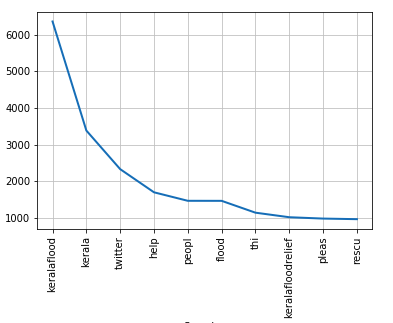
\includegraphics[scale=0.45]{fig_1.png}
  \end{center}
  
 \end{itemize}
\end{frame}

\begin{frame}[fragile]{ Implementations \& Results(Contd.)}

 \begin{itemize}
\item The TF-IDF vectorizer converts the tweets into
vectors when each tweets are processed and appended to a
list and this list was provided to the TF-IDF vectorizer.
\item .Further we used
K-Means clustering algorithm to group tweets into chosen
number (say, here five) of groups. The Output on using five
groups cluster we obtained is shown in Table I. 





 \end{itemize}
\end{frame}

\begin{frame}[fragile]{ Implementations \& Results(Contd.)}


\begin{table}[!htbp]
\centering
\begin{tabular}{|p{0.5cm}|p{4.5cm}| p{1cm}| } 
 \hline
0 & keralaflood, twitter, kerala, rescue, flood & 115 \\

 1 &  help, donate, people, please, need & 3925\\ 

 2 &chiefminister, minister, relief fund, crore & 72\\

  3 & children, feet long bridge, bridge rescue, citizen malampuzha, senior citizen malampuzha & 257\\ 

   4 & twitterkeralaflood, status, keralafloodrelief, keralaflood, kerala & 1824\\ 
 \hline
\end{tabular}
\label{tid}
\caption{\label{Kmeans}Five different groups with their respective hashtags}
\end{table}




\end{frame}


\begin{frame}[fragile]{ Implementations \& Results(Contd.)}

\textbf{3. Cluster-based \& topic modeling}

\begin{itemize}
\item K-means generates the following clusters for the K-value
5.
\begin{itemize}
\item Cluster 0: Words: alert district rain affect 
these district 
\item  Cluster 1: Words: announce person maharashtra serious
injury decrease
\item Cluster 2: Words: keralaflood kerala twitter help people
\item Cluster 3: Words: will keralaflood keralafloodrelief train
kerala
\item Cluster 4: Words: chief minister chief minister announce
announce crore
\end{itemize}

\end{itemize}




\end{frame}


\begin{frame}[fragile]{ Implementations \& Results(Contd.)}

\textbf{4. Topic Modeling Using LDA}

\begin{itemize}

\item A topic
model is a type of statistical model for discovering the abstract
”topics” that occur in a collection of documents  and used for text-processing as
it deduces the theme of texts . 
\item We implemented LDA
to identify the topic of the tweets, as shown in Table II.
\begin{table}[htbp]
	\centering
\begin{tabular}{ |p{0.8cm}|p{7.5cm}| } 
 \hline
 \textbf{Topics} & \textbf{Words(Clustered After Topic Modeling)}\\
 \hline
0 & keralaflood, kerala, nation, need, flood, relief \\
\hline
 1 &  keralaflood, twitter, family, rescue, flood, people \\ 
 \hline
 2 &keralaflood, twitter, kerala, rescue, water, operation\\
 \hline
  3 & keralaflood, road, twitter, ernakulam, near, please\\ 
  \hline
   4 & keralaflood, twitter, train, kerala, govern, keralafloodrelief\\ 
 \hline
\end{tabular}
\label{lda}
\caption{LDA output for five different topics}
\end{table}
\end{itemize}




\end{frame}


\begin{frame}[fragile]{ Implementations \& Results(Contd.)}

\begin{itemize}


\item The words are associated with each and every topic and they
represent certain meanings. Topic 0 is about Help, Topic 1 is
about Action, Topic 2 is somewhat similar to Topic 1,Topic 3 is
about Affected Location or Geography, Topic 4 is about Support
and so on other can be identified , etc.



\end{itemize}



\end{frame}




\section{Conclusions \& Future Works}
\begin{frame}[fragile]{ Conclusions \& Future Works}

\begin{itemize}


\item It is clear from the above analysis that how powerful a
social media is and social media can be harnessed
to great effect in times of crisis. 
\item Some of the steps which
are taken in this article are also adopted by twitter itself to
help surrounding community in fighting against disaster, crisis,
etc. \& Facebook also introduced a feature 'Mark-safe' to fight against these disasters. 
\item  We
will focus on making it more accurate and useful by applying
some Neural Network concepts in this project in future. 
\item To
make this system more powerful and useful, by implementing
some technique that can detect non-hashtag words that are
relevant for analysis.(E.g.- e ’People’
as ’ppl’ ).
\item Machine learning techniques
can be employed to check the veracity of social media by
comparing contents from actual news reports.


\end{itemize}



\end{frame}

\section{References}
\begin{frame}[fragile]{ References - I}
[1]. N. Saharia, “Detecting emotion from short messages on nepal earthquake,”
in \textit{Speech Technology and Human-Computer Dialogue (SpeD),
2015 International Conference on}. IEEE, 2015, pp. 1–5.\newline
[2]. S. Kedar, S. Owen, C. Jones, A. Donnelan, M. Glasscoe, and R. Duren,
“Select technologies and capabilities to improve earthquake resiliency in
california,” 2016.\newline
[3]. D. M. Blei, A. Y. Ng, and M. I. Jordan, “\textit{Latent dirichlet allocation,”
Journal of machine Learning research}, vol. 3, no. Jan, pp. 993–1022,
2003.\newline
[4]. J. A. Hartigan and M. A. Wong, “Algorithm as 136: A k-means clustering
algorithm,” \textit{Journal of the Royal Statistical Society. Series C (Applied
Statistics)}, vol. 28, no. 1, pp. 100–108, 1979.\newline
[5]. D. Hardt, “The oauth 2.0 authorization framework,” Tech. Rep., 2012.

 
 \end{frame}
 \begin{frame}[fragile]{ References - II}
[6]. H.-N. Teodorescu and N. Saharia, “An internet slang annotated dictionary
and its use in assessing message attitude and sentiments,” in \textit{Speech
Technology and Human-Computer Dialogue (SpeD), 2015 International
Conference on}. IEEE, 2015, pp. 1–8.\newline
[7]. G. Salton and C. Buckley, “Term-weighting approaches in automatic text
retrieval,” \textit{Information processing \& management}, vol. 24, no. 5, pp. 513–
523, 1988.\newline
[8]. H. M. Wallach, “Topic modeling: beyond bag-of-words,” in \textit{Proceedings
of the 23rd international conference on Machine learning}. ACM, 2006,
pp. 977–984.
 \end{frame}
 
\section{Source data Repository}
\begin{frame}[fragile]{Source data Repository}
\begin{itemize}
\item Source code and Dataset for this Project can be found at -
\href{https://www.github.com}{ Here (Github)} 
\end{itemize}

 \end{frame}
 \section{Thank You}
 
 
\end{document}
